\documentclass[1p]{elsarticle_modified}
%\bibliographystyle{elsarticle-num}

%\usepackage[colorlinks]{hyperref}
%\usepackage{abbrmath_seonhwa} %\Abb, \Ascr, \Acal ,\Abf, \Afrak
\usepackage{amsfonts}
\usepackage{amssymb}
\usepackage{amsmath}
\usepackage{amsthm}
\usepackage{scalefnt}
\usepackage{amsbsy}
\usepackage{kotex}
\usepackage{caption}
\usepackage{subfig}
\usepackage{color}
\usepackage{graphicx}
\usepackage{xcolor} %% white, black, red, green, blue, cyan, magenta, yellow
\usepackage{float}
\usepackage{setspace}
\usepackage{hyperref}

\usepackage{tikz}
\usetikzlibrary{arrows}

\usepackage{multirow}
\usepackage{array} % fixed length table
\usepackage{hhline}

%%%%%%%%%%%%%%%%%%%%%
\makeatletter
\renewcommand*\env@matrix[1][\arraystretch]{%
	\edef\arraystretch{#1}%
	\hskip -\arraycolsep
	\let\@ifnextchar\new@ifnextchar
	\array{*\c@MaxMatrixCols c}}
\makeatother %https://tex.stackexchange.com/questions/14071/how-can-i-increase-the-line-spacing-in-a-matrix
%%%%%%%%%%%%%%%

\usepackage[normalem]{ulem}

\newcommand{\msout}[1]{\ifmmode\text{\sout{\ensuremath{#1}}}\else\sout{#1}\fi}
%SOURCE: \msout is \stkout macro in https://tex.stackexchange.com/questions/20609/strikeout-in-math-mode

\newcommand{\cancel}[1]{
	\ifmmode
	{\color{red}\msout{#1}}
	\else
	{\color{red}\sout{#1}}
	\fi
}

\newcommand{\add}[1]{
	{\color{blue}\uwave{#1}}
}

\newcommand{\replace}[2]{
	\ifmmode
	{\color{red}\msout{#1}}{\color{blue}\uwave{#2}}
	\else
	{\color{red}\sout{#1}}{\color{blue}\uwave{#2}}
	\fi
}

\newcommand{\Sol}{\mathcal{S}} %segment
\newcommand{\D}{D} %diagram
\newcommand{\A}{\mathcal{A}} %arc


%%%%%%%%%%%%%%%%%%%%%%%%%%%%%5 test

\def\sl{\operatorname{\textup{SL}}(2,\Cbb)}
\def\psl{\operatorname{\textup{PSL}}(2,\Cbb)}
\def\quan{\mkern 1mu \triangleright \mkern 1mu}

\theoremstyle{definition}
\newtheorem{thm}{Theorem}[section]
\newtheorem{prop}[thm]{Proposition}
\newtheorem{lem}[thm]{Lemma}
\newtheorem{ques}[thm]{Question}
\newtheorem{cor}[thm]{Corollary}
\newtheorem{defn}[thm]{Definition}
\newtheorem{exam}[thm]{Example}
\newtheorem{rmk}[thm]{Remark}
\newtheorem{alg}[thm]{Algorithm}

\newcommand{\I}{\sqrt{-1}}
\begin{document}

%\begin{frontmatter}
%
%\title{Boundary parabolic representations of knots up to 8 crossings}
%
%%% Group authors per affiliation:
%\author{Yunhi Cho} 
%\address{Department of Mathematics, University of Seoul, Seoul, Korea}
%\ead{yhcho@uos.ac.kr}
%
%
%\author{Seonhwa Kim} %\fnref{s_kim}}
%\address{Center for Geometry and Physics, Institute for Basic Science, Pohang, 37673, Korea}
%\ead{ryeona17@ibs.re.kr}
%
%\author{Hyuk Kim}
%\address{Department of Mathematical Sciences, Seoul National University, Seoul 08826, Korea}
%\ead{hyukkim@snu.ac.kr}
%
%\author{Seokbeom Yoon}
%\address{Department of Mathematical Sciences, Seoul National University, Seoul, 08826,  Korea}
%\ead{sbyoon15@snu.ac.kr}
%
%\begin{abstract}
%We find all boundary parabolic representation of knots up to 8 crossings.
%
%\end{abstract}
%\begin{keyword}
%    \MSC[2010] 57M25 
%\end{keyword}
%
%\end{frontmatter}

%\linenumbers
%\tableofcontents
%
\newcommand\colored[1]{\textcolor{white}{\rule[-0.35ex]{0.8em}{1.4ex}}\kern-0.8em\color{red} #1}%
%\newcommand\colored[1]{\textcolor{white}{ #1}\kern-2.17ex	\textcolor{white}{ #1}\kern-1.81ex	\textcolor{white}{ #1}\kern-2.15ex\color{red}#1	}

{\Large $\underline{12n_{0007}~(K12n_{0007})}$}

\setlength{\tabcolsep}{10pt}
\renewcommand{\arraystretch}{1.6}
\vspace{1cm}\begin{tabular}{m{100pt}>{\centering\arraybackslash}m{274pt}}
\multirow{5}{120pt}{
	\centering
	\includegraphics[width=112pt]{../../../GIT/diagram.site/Diagrams/png/2096_12n_0007.png}\\
\ \ \ A knot diagram\footnotemark}&
\allowdisplaybreaks
\textbf{Linearized knot diagam} \\
\cline{2-2}
 &
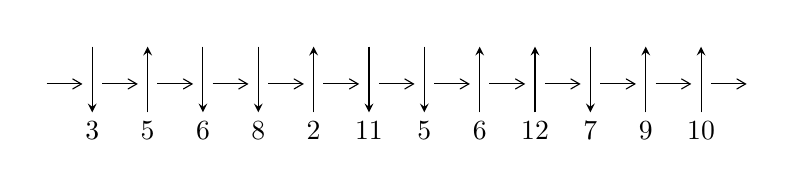
\begin{tikzpicture}[x=20pt, y=17pt]
	% nodes
	\node (C0) at (0, 0) {};
	\node (C1) at (1, 0) {};
	\node (C1U) at (1, +1) {};
	\node (C1D) at (1, -1) {3};

	\node (C2) at (2, 0) {};
	\node (C2U) at (2, +1) {};
	\node (C2D) at (2, -1) {5};

	\node (C3) at (3, 0) {};
	\node (C3U) at (3, +1) {};
	\node (C3D) at (3, -1) {6};

	\node (C4) at (4, 0) {};
	\node (C4U) at (4, +1) {};
	\node (C4D) at (4, -1) {8};

	\node (C5) at (5, 0) {};
	\node (C5U) at (5, +1) {};
	\node (C5D) at (5, -1) {2};

	\node (C6) at (6, 0) {};
	\node (C6U) at (6, +1) {};
	\node (C6D) at (6, -1) {11};

	\node (C7) at (7, 0) {};
	\node (C7U) at (7, +1) {};
	\node (C7D) at (7, -1) {5};

	\node (C8) at (8, 0) {};
	\node (C8U) at (8, +1) {};
	\node (C8D) at (8, -1) {6};

	\node (C9) at (9, 0) {};
	\node (C9U) at (9, +1) {};
	\node (C9D) at (9, -1) {12};

	\node (C10) at (10, 0) {};
	\node (C10U) at (10, +1) {};
	\node (C10D) at (10, -1) {7};

	\node (C11) at (11, 0) {};
	\node (C11U) at (11, +1) {};
	\node (C11D) at (11, -1) {9};

	\node (C12) at (12, 0) {};
	\node (C12U) at (12, +1) {};
	\node (C12D) at (12, -1) {10};
	\node (C13) at (13, 0) {};

	% arrows
	\draw[->,>={angle 60}]
	(C0) edge (C1) (C1) edge (C2) (C2) edge (C3) (C3) edge (C4) (C4) edge (C5) (C5) edge (C6) (C6) edge (C7) (C7) edge (C8) (C8) edge (C9) (C9) edge (C10) (C10) edge (C11) (C11) edge (C12) (C12) edge (C13) ;	\draw[->,>=stealth]
	(C1U) edge (C1D) (C2D) edge (C2U) (C3U) edge (C3D) (C4U) edge (C4D) (C5D) edge (C5U) (C6U) edge (C6D) (C7U) edge (C7D) (C8D) edge (C8U) (C9D) edge (C9U) (C10U) edge (C10D) (C11D) edge (C11U) (C12D) edge (C12U) ;
	\end{tikzpicture} \\
\hhline{~~} \\& 
\textbf{Solving Sequence} \\ \cline{2-2} 
 &
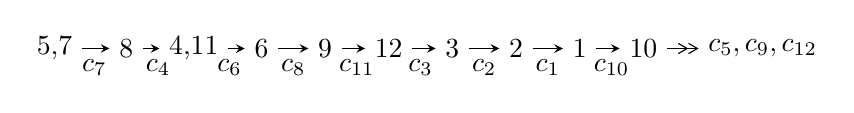
\begin{tikzpicture}[x=23pt, y=7pt]
	% node
	\node (A0) at (-1/8, 0) {5,7};
	\node (A1) at (1, 0) {8};
	\node (A2) at (33/16, 0) {4,11};
	\node (A3) at (25/8, 0) {6};
	\node (A4) at (33/8, 0) {9};
	\node (A5) at (41/8, 0) {12};
	\node (A6) at (49/8, 0) {3};
	\node (A7) at (57/8, 0) {2};
	\node (A8) at (65/8, 0) {1};
	\node (A9) at (73/8, 0) {10};
	\node (C1) at (1/2, -1) {$c_{7}$};
	\node (C2) at (3/2, -1) {$c_{4}$};
	\node (C3) at (21/8, -1) {$c_{6}$};
	\node (C4) at (29/8, -1) {$c_{8}$};
	\node (C5) at (37/8, -1) {$c_{11}$};
	\node (C6) at (45/8, -1) {$c_{3}$};
	\node (C7) at (53/8, -1) {$c_{2}$};
	\node (C8) at (61/8, -1) {$c_{1}$};
	\node (C9) at (69/8, -1) {$c_{10}$};
	\node (A10) at (11, 0) {$c_{5},c_{9},c_{12}$};

	% edge
	\draw[->,>=stealth]	
	(A0) edge (A1) (A1) edge (A2) (A2) edge (A3) (A3) edge (A4) (A4) edge (A5) (A5) edge (A6) (A6) edge (A7) (A7) edge (A8) (A8) edge (A9) ;
	\draw[->>,>={angle 60}]	
	(A9) edge (A10);
\end{tikzpicture} \\ 

\end{tabular} \\

\footnotetext{
The image of knot diagram is generated by the software ``\textbf{Draw programme}" developed by Andrew Bartholomew(\url{http://www.layer8.co.uk/maths/draw/index.htm\#Running-draw}), where we modified some parts for our purpose(\url{https://github.com/CATsTAILs/LinksPainter}).
}\phantom \\ \newline 
\centering \textbf{Ideals for irreducible components\footnotemark of $X_{\text{par}}$} 
 
\begin{align*}
I^u_{1}&=\langle 
-9.22578\times10^{81} u^{32}+2.64829\times10^{82} u^{31}+\cdots+1.74190\times10^{85} b+7.65657\times10^{83},\\
\phantom{I^u_{1}}&\phantom{= \langle  }1.64277\times10^{83} u^{32}-4.01664\times10^{83} u^{31}+\cdots+6.96761\times10^{85} a-2.63055\times10^{86},\\
\phantom{I^u_{1}}&\phantom{= \langle  }u^{33}-2 u^{32}+\cdots-1024 u^2+1024\rangle \\
I^u_{2}&=\langle 
b,\;-2 u^3- u^2+a-5 u-1,\;u^4+u^3+3 u^2+2 u+1\rangle \\
\\
I^v_{1}&=\langle 
a,\;-152 v^9+36 v^8-216 v^7+881 v^6-468 v^5+684 v^4-1376 v^3+252 v^2+115 b-144 v+219,\\
\phantom{I^v_{1}}&\phantom{= \langle  }v^{10}- v^9+2 v^8-7 v^7+8 v^6-9 v^5+14 v^4-10 v^3+5 v^2-3 v+1\rangle \\
\end{align*}
\raggedright * 3 irreducible components of $\dim_{\mathbb{C}}=0$, with total 47 representations.\\
\footnotetext{All coefficients of polynomials are rational numbers. But the coefficients are sometimes approximated in decimal forms when there is not enough margin.}
\newpage
\renewcommand{\arraystretch}{1}
\centering \section*{I. $I^u_{1}= \langle -9.23\times10^{81} u^{32}+2.65\times10^{82} u^{31}+\cdots+1.74\times10^{85} b+7.66\times10^{83},\;1.64\times10^{83} u^{32}-4.02\times10^{83} u^{31}+\cdots+6.97\times10^{85} a-2.63\times10^{86},\;u^{33}-2 u^{32}+\cdots-1024 u^2+1024 \rangle$}
\flushleft \textbf{(i) Arc colorings}\\
\begin{tabular}{m{7pt} m{180pt} m{7pt} m{180pt} }
\flushright $a_{5}=$&$\begin{pmatrix}0\\u\end{pmatrix}$ \\
\flushright $a_{7}=$&$\begin{pmatrix}1\\0\end{pmatrix}$ \\
\flushright $a_{8}=$&$\begin{pmatrix}1\\u^2\end{pmatrix}$ \\
\flushright $a_{4}=$&$\begin{pmatrix}u\\u^3+u\end{pmatrix}$ \\
\flushright $a_{11}=$&$\begin{pmatrix}-0.00235772 u^{32}+0.00576474 u^{31}+\cdots-1.78671 u+3.77540\\0.000529638 u^{32}-0.00152034 u^{31}+\cdots+1.75463 u-0.0439552\end{pmatrix}$ \\
\flushright $a_{6}=$&$\begin{pmatrix}0.00161857 u^{32}-0.00336873 u^{31}+\cdots-4.32267 u+2.88182\\-0.000754427 u^{32}+0.00172427 u^{31}+\cdots+0.455492 u-1.26583\end{pmatrix}$ \\
\flushright $a_{9}=$&$\begin{pmatrix}0.000947588 u^{32}-0.00205444 u^{31}+\cdots-0.758148 u+2.00893\\0.000267518 u^{32}-0.000630392 u^{31}+\cdots+0.294022 u+0.443178\end{pmatrix}$ \\
\flushright $a_{12}=$&$\begin{pmatrix}-0.00169931 u^{32}+0.00435099 u^{31}+\cdots-3.09719 u+4.67643\\0.000267518 u^{32}-0.000630392 u^{31}+\cdots+0.294022 u+0.443178\end{pmatrix}$ \\
\flushright $a_{3}=$&$\begin{pmatrix}-0.00169705 u^{32}+0.00482151 u^{31}+\cdots+0.535570 u-2.78065\\-0.000159267 u^{32}+0.000118296 u^{31}+\cdots+2.00893 u-0.970330\end{pmatrix}$ \\
\flushright $a_{2}=$&$\begin{pmatrix}-0.00169705 u^{32}+0.00482151 u^{31}+\cdots+0.535570 u-2.78065\\0.0000201791 u^{32}-0.000817233 u^{31}+\cdots+3.74671 u-2.43201\end{pmatrix}$ \\
\flushright $a_{1}=$&$\begin{pmatrix}-0.00167929 u^{32}+0.00313362 u^{31}+\cdots+6.43558 u-4.28239\\-0.0000607181 u^{32}-0.000235106 u^{31}+\cdots+2.11291 u-1.40057\end{pmatrix}$ \\
\flushright $a_{10}=$&$\begin{pmatrix}-0.00182808 u^{32}+0.00424440 u^{31}+\cdots-0.0320791 u+3.73144\\0.000529638 u^{32}-0.00152034 u^{31}+\cdots+1.75463 u-0.0439552\end{pmatrix}$\\&\end{tabular}
\flushleft \textbf{(ii) Obstruction class $= -1$}\\~\\
\flushleft \textbf{(iii) Cusp Shapes $= -0.00699839 u^{32}+0.0259705 u^{31}+\cdots-24.8101 u+1.26303$}\\~\\
\newpage\renewcommand{\arraystretch}{1}
\flushleft \textbf{(iv) u-Polynomials at the component}\newline \\
\begin{tabular}{m{50pt}|m{274pt}}
Crossings & \hspace{64pt}u-Polynomials at each crossing \\
\hline $$\begin{aligned}c_{1}\end{aligned}$$&$\begin{aligned}
&u^{33}+5 u^{32}+\cdots+3 u-1
\end{aligned}$\\
\hline $$\begin{aligned}c_{2},c_{5}\end{aligned}$$&$\begin{aligned}
&u^{33}+7 u^{32}+\cdots+5 u+1
\end{aligned}$\\
\hline $$\begin{aligned}c_{3}\end{aligned}$$&$\begin{aligned}
&u^{33}-7 u^{32}+\cdots-29960 u+14308
\end{aligned}$\\
\hline $$\begin{aligned}c_{4},c_{7}\end{aligned}$$&$\begin{aligned}
&u^{33}-2 u^{32}+\cdots-1024 u^2+1024
\end{aligned}$\\
\hline $$\begin{aligned}c_{6},c_{10}\end{aligned}$$&$\begin{aligned}
&u^{33}+3 u^{32}+\cdots+56 u-16
\end{aligned}$\\
\hline $$\begin{aligned}c_{8}\end{aligned}$$&$\begin{aligned}
&u^{33}+4 u^{32}+\cdots+2 u+1
\end{aligned}$\\
\hline $$\begin{aligned}c_{9},c_{11},c_{12}\end{aligned}$$&$\begin{aligned}
&u^{33}+7 u^{32}+\cdots+4 u-1
\end{aligned}$\\
\hline
\end{tabular}\\~\\
\newpage\renewcommand{\arraystretch}{1}
\flushleft \textbf{(v) Riley Polynomials at the component}\newline \\
\begin{tabular}{m{50pt}|m{274pt}}
Crossings & \hspace{64pt}Riley Polynomials at each crossing \\
\hline $$\begin{aligned}c_{1}\end{aligned}$$&$\begin{aligned}
&y^{33}+53 y^{32}+\cdots+3 y-1
\end{aligned}$\\
\hline $$\begin{aligned}c_{2},c_{5}\end{aligned}$$&$\begin{aligned}
&y^{33}+5 y^{32}+\cdots+3 y-1
\end{aligned}$\\
\hline $$\begin{aligned}c_{3}\end{aligned}$$&$\begin{aligned}
&y^{33}+101 y^{32}+\cdots+162370712 y-204718864
\end{aligned}$\\
\hline $$\begin{aligned}c_{4},c_{7}\end{aligned}$$&$\begin{aligned}
&y^{33}+60 y^{32}+\cdots+2097152 y-1048576
\end{aligned}$\\
\hline $$\begin{aligned}c_{6},c_{10}\end{aligned}$$&$\begin{aligned}
&y^{33}+33 y^{32}+\cdots-2496 y-256
\end{aligned}$\\
\hline $$\begin{aligned}c_{8}\end{aligned}$$&$\begin{aligned}
&y^{33}-62 y^{32}+\cdots-26 y-1
\end{aligned}$\\
\hline $$\begin{aligned}c_{9},c_{11},c_{12}\end{aligned}$$&$\begin{aligned}
&y^{33}-39 y^{32}+\cdots-124 y-1
\end{aligned}$\\
\hline
\end{tabular}\\~\\
\newpage\flushleft \textbf{(vi) Complex Volumes and Cusp Shapes}
$$\begin{array}{c|c|c}  
\text{Solutions to }I^u_{1}& \I (\text{vol} + \sqrt{-1}CS) & \text{Cusp shape}\\
 \hline 
\begin{aligned}
u &= -0.736102 + 0.542727 I \\
a &= -0.637804 - 0.145676 I \\
b &= -0.263754 + 1.251930 I\end{aligned}
 & \phantom{-}4.58725 + 2.79647 I & \phantom{-}1.21032 - 3.36441 I \\ \hline\begin{aligned}
u &= -0.736102 - 0.542727 I \\
a &= -0.637804 + 0.145676 I \\
b &= -0.263754 - 1.251930 I\end{aligned}
 & \phantom{-}4.58725 - 2.79647 I & \phantom{-}1.21032 + 3.36441 I \\ \hline\begin{aligned}
u &= \phantom{-}0.624216 + 0.614071 I \\
a &= -0.451815 - 0.151872 I \\
b &= -0.581770 + 1.231250 I\end{aligned}
 & \phantom{-}6.44848 + 5.59696 I & \phantom{-}6.32857 - 1.76937 I \\ \hline\begin{aligned}
u &= \phantom{-}0.624216 - 0.614071 I \\
a &= -0.451815 + 0.151872 I \\
b &= -0.581770 - 1.231250 I\end{aligned}
 & \phantom{-}6.44848 - 5.59696 I & \phantom{-}6.32857 + 1.76937 I \\ \hline\begin{aligned}
u &= \phantom{-}0.296890 + 0.749665 I \\
a &= -0.46200 - 1.54808 I \\
b &= -0.396918 + 0.657378 I\end{aligned}
 & \phantom{-}2.07164 - 0.96578 I & \phantom{-}7.05787 - 0.04324 I \\ \hline\begin{aligned}
u &= \phantom{-}0.296890 - 0.749665 I \\
a &= -0.46200 + 1.54808 I \\
b &= -0.396918 - 0.657378 I\end{aligned}
 & \phantom{-}2.07164 + 0.96578 I & \phantom{-}7.05787 + 0.04324 I \\ \hline\begin{aligned}
u &= -0.479019 + 0.528772 I \\
a &= \phantom{-}2.34330 + 1.85274 I \\
b &= \phantom{-}0.056157 - 0.749682 I\end{aligned}
 & \phantom{-}1.16540 - 2.90676 I & \phantom{-}5.52935 + 0.45206 I \\ \hline\begin{aligned}
u &= -0.479019 - 0.528772 I \\
a &= \phantom{-}2.34330 - 1.85274 I \\
b &= \phantom{-}0.056157 + 0.749682 I\end{aligned}
 & \phantom{-}1.16540 + 2.90676 I & \phantom{-}5.52935 - 0.45206 I \\ \hline\begin{aligned}
u &= \phantom{-}0.639723 + 0.300028 I \\
a &= \phantom{-}0.463444 + 0.633798 I \\
b &= \phantom{-}0.345995 - 0.989797 I\end{aligned}
 & \phantom{-}0.62465 + 2.03384 I & \phantom{-}1.49443 - 2.77231 I \\ \hline\begin{aligned}
u &= \phantom{-}0.639723 - 0.300028 I \\
a &= \phantom{-}0.463444 - 0.633798 I \\
b &= \phantom{-}0.345995 + 0.989797 I\end{aligned}
 & \phantom{-}0.62465 - 2.03384 I & \phantom{-}1.49443 + 2.77231 I\\
 \hline 
 \end{array}$$\newpage$$\begin{array}{c|c|c}  
\text{Solutions to }I^u_{1}& \I (\text{vol} + \sqrt{-1}CS) & \text{Cusp shape}\\
 \hline 
\begin{aligned}
u &= -0.680743\phantom{ +0.000000I} \\
a &= -1.22755\phantom{ +0.000000I} \\
b &= -0.999659\phantom{ +0.000000I}\end{aligned}
 & \phantom{-}2.80941\phantom{ +0.000000I} & \phantom{-}2.91480\phantom{ +0.000000I} \\ \hline\begin{aligned}
u &= -0.445593 + 0.510958 I \\
a &= \phantom{-}0.788593 + 0.405247 I \\
b &= \phantom{-}0.389650 - 0.507994 I\end{aligned}
 & -0.634147 + 1.259730 I & -4.30303 - 4.77679 I \\ \hline\begin{aligned}
u &= -0.445593 - 0.510958 I \\
a &= \phantom{-}0.788593 - 0.405247 I \\
b &= \phantom{-}0.389650 + 0.507994 I\end{aligned}
 & -0.634147 - 1.259730 I & -4.30303 + 4.77679 I \\ \hline\begin{aligned}
u &= -0.304293 + 0.498677 I \\
a &= \phantom{-}1.074760 - 0.330459 I \\
b &= -0.237073 - 0.267230 I\end{aligned}
 & -0.29538 + 1.55166 I & -2.33060 - 5.33546 I \\ \hline\begin{aligned}
u &= -0.304293 - 0.498677 I \\
a &= \phantom{-}1.074760 + 0.330459 I \\
b &= -0.237073 + 0.267230 I\end{aligned}
 & -0.29538 - 1.55166 I & -2.33060 + 5.33546 I \\ \hline\begin{aligned}
u &= \phantom{-}0.529499 + 0.187441 I \\
a &= \phantom{-}4.29355 - 1.67102 I \\
b &= \phantom{-}0.312701 + 0.419841 I\end{aligned}
 & \phantom{-}1.84801 - 1.60722 I & \phantom{-}0.8190 + 15.0118 I \\ \hline\begin{aligned}
u &= \phantom{-}0.529499 - 0.187441 I \\
a &= \phantom{-}4.29355 + 1.67102 I \\
b &= \phantom{-}0.312701 - 0.419841 I\end{aligned}
 & \phantom{-}1.84801 + 1.60722 I & \phantom{-}0.8190 - 15.0118 I \\ \hline\begin{aligned}
u &= -0.10031 + 1.67720 I \\
a &= -0.0503517 - 0.0297636 I \\
b &= -0.604916 + 0.020460 I\end{aligned}
 & \phantom{-}7.91587 + 3.25842 I & \phantom{-0.000000 } 0 \\ \hline\begin{aligned}
u &= -0.10031 - 1.67720 I \\
a &= -0.0503517 + 0.0297636 I \\
b &= -0.604916 - 0.020460 I\end{aligned}
 & \phantom{-}7.91587 - 3.25842 I & \phantom{-0.000000 } 0 \\ \hline\begin{aligned}
u &= -0.85403 + 1.58938 I \\
a &= -0.454673 - 0.911109 I \\
b &= \phantom{-}0.21829 + 1.69561 I\end{aligned}
 & \phantom{-}9.42003 - 4.56175 I & \phantom{-0.000000 } 0\\
 \hline 
 \end{array}$$\newpage$$\begin{array}{c|c|c}  
\text{Solutions to }I^u_{1}& \I (\text{vol} + \sqrt{-1}CS) & \text{Cusp shape}\\
 \hline 
\begin{aligned}
u &= -0.85403 - 1.58938 I \\
a &= -0.454673 + 0.911109 I \\
b &= \phantom{-}0.21829 - 1.69561 I\end{aligned}
 & \phantom{-}9.42003 + 4.56175 I & \phantom{-0.000000 } 0 \\ \hline\begin{aligned}
u &= \phantom{-}1.61914 + 1.36310 I \\
a &= -0.415764 + 0.566639 I \\
b &= -0.06793 - 1.82415 I\end{aligned}
 & \phantom{-}11.88220 - 1.87850 I & \phantom{-0.000000 } 0 \\ \hline\begin{aligned}
u &= \phantom{-}1.61914 - 1.36310 I \\
a &= -0.415764 - 0.566639 I \\
b &= -0.06793 + 1.82415 I\end{aligned}
 & \phantom{-}11.88220 + 1.87850 I & \phantom{-0.000000 } 0 \\ \hline\begin{aligned}
u &= \phantom{-}0.47200 + 2.29182 I \\
a &= -0.313254 + 1.103940 I \\
b &= -0.34561 - 1.60946 I\end{aligned}
 & \phantom{-}13.8782 - 7.1833 I & \phantom{-0.000000 } 0 \\ \hline\begin{aligned}
u &= \phantom{-}0.47200 - 2.29182 I \\
a &= -0.313254 - 1.103940 I \\
b &= -0.34561 + 1.60946 I\end{aligned}
 & \phantom{-}13.8782 + 7.1833 I & \phantom{-0.000000 } 0 \\ \hline\begin{aligned}
u &= \phantom{-}0.91656 + 2.15918 I \\
a &= \phantom{-}0.567229 - 0.874265 I \\
b &= \phantom{-}0.84459 + 1.62798 I\end{aligned}
 & -18.3854 - 12.6657 I & \phantom{-0.000000 } 0 \\ \hline\begin{aligned}
u &= \phantom{-}0.91656 - 2.15918 I \\
a &= \phantom{-}0.567229 + 0.874265 I \\
b &= \phantom{-}0.84459 - 1.62798 I\end{aligned}
 & -18.3854 + 12.6657 I & \phantom{-0.000000 } 0 \\ \hline\begin{aligned}
u &= \phantom{-}0.01301 + 2.40418 I \\
a &= -0.078585 - 1.110070 I \\
b &= -0.18185 + 1.65385 I\end{aligned}
 & \phantom{-}14.1748 - 0.2842 I & \phantom{-0.000000 } 0 \\ \hline\begin{aligned}
u &= \phantom{-}0.01301 - 2.40418 I \\
a &= -0.078585 + 1.110070 I \\
b &= -0.18185 - 1.65385 I\end{aligned}
 & \phantom{-}14.1748 + 0.2842 I & \phantom{-0.000000 } 0 \\ \hline\begin{aligned}
u &= -0.27091 + 2.43864 I \\
a &= \phantom{-}0.0842297 + 0.0547107 I \\
b &= \phantom{-}1.72368 + 0.09458 I\end{aligned}
 & \phantom{-}16.4290 + 3.7881 I & \phantom{-0.000000 } 0\\
 \hline 
 \end{array}$$\newpage$$\begin{array}{c|c|c}  
\text{Solutions to }I^u_{1}& \I (\text{vol} + \sqrt{-1}CS) & \text{Cusp shape}\\
 \hline 
\begin{aligned}
u &= -0.27091 - 2.43864 I \\
a &= \phantom{-}0.0842297 - 0.0547107 I \\
b &= \phantom{-}1.72368 - 0.09458 I\end{aligned}
 & \phantom{-}16.4290 - 3.7881 I & \phantom{-0.000000 } 0 \\ \hline\begin{aligned}
u &= -0.58040 + 2.51179 I \\
a &= \phantom{-}0.362910 + 0.854969 I \\
b &= \phantom{-}0.78859 - 1.76638 I\end{aligned}
 & -17.4300 + 5.1499 I & \phantom{-0.000000 } 0 \\ \hline\begin{aligned}
u &= -0.58040 - 2.51179 I \\
a &= \phantom{-}0.362910 - 0.854969 I \\
b &= \phantom{-}0.78859 + 1.76638 I\end{aligned}
 & -17.4300 - 5.1499 I & \phantom{-0.000000 } 0\\
 \hline 
 \end{array}$$\newpage\newpage\renewcommand{\arraystretch}{1}
\centering \section*{II. $I^u_{2}= \langle b,\;-2 u^3- u^2+a-5 u-1,\;u^4+u^3+3 u^2+2 u+1 \rangle$}
\flushleft \textbf{(i) Arc colorings}\\
\begin{tabular}{m{7pt} m{180pt} m{7pt} m{180pt} }
\flushright $a_{5}=$&$\begin{pmatrix}0\\u\end{pmatrix}$ \\
\flushright $a_{7}=$&$\begin{pmatrix}1\\0\end{pmatrix}$ \\
\flushright $a_{8}=$&$\begin{pmatrix}1\\u^2\end{pmatrix}$ \\
\flushright $a_{4}=$&$\begin{pmatrix}u\\u^3+u\end{pmatrix}$ \\
\flushright $a_{11}=$&$\begin{pmatrix}2 u^3+u^2+5 u+1\\0\end{pmatrix}$ \\
\flushright $a_{6}=$&$\begin{pmatrix}1\\0\end{pmatrix}$ \\
\flushright $a_{9}=$&$\begin{pmatrix}u^2+1\\u^2\end{pmatrix}$ \\
\flushright $a_{12}=$&$\begin{pmatrix}2 u^3+5 u\\- u^2\end{pmatrix}$ \\
\flushright $a_{3}=$&$\begin{pmatrix}u^3+2 u\\u^3+u\end{pmatrix}$ \\
\flushright $a_{2}=$&$\begin{pmatrix}u^3+2 u\\u^3+u^2+2 u+1\end{pmatrix}$ \\
\flushright $a_{1}=$&$\begin{pmatrix}- u^2-1\\- u^2\end{pmatrix}$ \\
\flushright $a_{10}=$&$\begin{pmatrix}2 u^3+u^2+5 u+1\\0\end{pmatrix}$\\&\end{tabular}
\flushleft \textbf{(ii) Obstruction class $= 1$}\\~\\
\flushleft \textbf{(iii) Cusp Shapes $= -8 u^3-11 u^2-22 u-11$}\\~\\
\newpage\renewcommand{\arraystretch}{1}
\flushleft \textbf{(iv) u-Polynomials at the component}\newline \\
\begin{tabular}{m{50pt}|m{274pt}}
Crossings & \hspace{64pt}u-Polynomials at each crossing \\
\hline $$\begin{aligned}c_{1},c_{4}\end{aligned}$$&$\begin{aligned}
&u^4- u^3+3 u^2-2 u+1
\end{aligned}$\\
\hline $$\begin{aligned}c_{2}\end{aligned}$$&$\begin{aligned}
&u^4- u^3+u^2+1
\end{aligned}$\\
\hline $$\begin{aligned}c_{3}\end{aligned}$$&$\begin{aligned}
&u^4+u^3+5 u^2- u+2
\end{aligned}$\\
\hline $$\begin{aligned}c_{5}\end{aligned}$$&$\begin{aligned}
&u^4+u^3+u^2+1
\end{aligned}$\\
\hline $$\begin{aligned}c_{6},c_{10}\end{aligned}$$&$\begin{aligned}
&u^4
\end{aligned}$\\
\hline $$\begin{aligned}c_{7}\end{aligned}$$&$\begin{aligned}
&u^4+u^3+3 u^2+2 u+1
\end{aligned}$\\
\hline $$\begin{aligned}c_{8}\end{aligned}$$&$\begin{aligned}
&u^4-5 u^3+7 u^2-2 u+1
\end{aligned}$\\
\hline $$\begin{aligned}c_{9}\end{aligned}$$&$\begin{aligned}
&(u+1)^4
\end{aligned}$\\
\hline $$\begin{aligned}c_{11},c_{12}\end{aligned}$$&$\begin{aligned}
&(u-1)^4
\end{aligned}$\\
\hline
\end{tabular}\\~\\
\newpage\renewcommand{\arraystretch}{1}
\flushleft \textbf{(v) Riley Polynomials at the component}\newline \\
\begin{tabular}{m{50pt}|m{274pt}}
Crossings & \hspace{64pt}Riley Polynomials at each crossing \\
\hline $$\begin{aligned}c_{1},c_{4},c_{7}\end{aligned}$$&$\begin{aligned}
&y^4+5 y^3+7 y^2+2 y+1
\end{aligned}$\\
\hline $$\begin{aligned}c_{2},c_{5}\end{aligned}$$&$\begin{aligned}
&y^4+y^3+3 y^2+2 y+1
\end{aligned}$\\
\hline $$\begin{aligned}c_{3}\end{aligned}$$&$\begin{aligned}
&y^4+9 y^3+31 y^2+19 y+4
\end{aligned}$\\
\hline $$\begin{aligned}c_{6},c_{10}\end{aligned}$$&$\begin{aligned}
&y^4
\end{aligned}$\\
\hline $$\begin{aligned}c_{8}\end{aligned}$$&$\begin{aligned}
&y^4-11 y^3+31 y^2+10 y+1
\end{aligned}$\\
\hline $$\begin{aligned}c_{9},c_{11},c_{12}\end{aligned}$$&$\begin{aligned}
&(y-1)^4
\end{aligned}$\\
\hline
\end{tabular}\\~\\
\newpage\flushleft \textbf{(vi) Complex Volumes and Cusp Shapes}
$$\begin{array}{c|c|c}  
\text{Solutions to }I^u_{2}& \I (\text{vol} + \sqrt{-1}CS) & \text{Cusp shape}\\
 \hline 
\begin{aligned}
u &= -0.395123 + 0.506844 I \\
a &= -0.59074 + 2.34806 I \\
b &= \phantom{-0.000000 } 0\end{aligned}
 & \phantom{-}1.43393 + 1.41510 I & -3.14142 - 7.60220 I \\ \hline\begin{aligned}
u &= -0.395123 - 0.506844 I \\
a &= -0.59074 - 2.34806 I \\
b &= \phantom{-0.000000 } 0\end{aligned}
 & \phantom{-}1.43393 - 1.41510 I & -3.14142 + 7.60220 I \\ \hline\begin{aligned}
u &= -0.10488 + 1.55249 I \\
a &= -0.409261 + 0.055548 I \\
b &= \phantom{-0.000000 } 0\end{aligned}
 & \phantom{-}8.43568 + 3.16396 I & \phantom{-}11.64142 - 1.04769 I \\ \hline\begin{aligned}
u &= -0.10488 - 1.55249 I \\
a &= -0.409261 - 0.055548 I \\
b &= \phantom{-0.000000 } 0\end{aligned}
 & \phantom{-}8.43568 - 3.16396 I & \phantom{-}11.64142 + 1.04769 I\\
 \hline 
 \end{array}$$\newpage\newpage\renewcommand{\arraystretch}{1}
\centering \section*{III. $I^v_{1}= \langle a,\;-152 v^9+36 v^8+\cdots+115 b+219,\;v^{10}- v^9+\cdots-3 v+1 \rangle$}
\flushleft \textbf{(i) Arc colorings}\\
\begin{tabular}{m{7pt} m{180pt} m{7pt} m{180pt} }
\flushright $a_{5}=$&$\begin{pmatrix}v\\0\end{pmatrix}$ \\
\flushright $a_{7}=$&$\begin{pmatrix}1\\0\end{pmatrix}$ \\
\flushright $a_{8}=$&$\begin{pmatrix}1\\0\end{pmatrix}$ \\
\flushright $a_{4}=$&$\begin{pmatrix}v\\0\end{pmatrix}$ \\
\flushright $a_{11}=$&$\begin{pmatrix}0\\1.32174 v^{9}-0.313043 v^{8}+\cdots+1.25217 v-1.90435\end{pmatrix}$ \\
\flushright $a_{6}=$&$\begin{pmatrix}1\\1.35652 v^{9}-0.373913 v^{8}+\cdots+1.49565 v-0.191304\end{pmatrix}$ \\
\flushright $a_{9}=$&$\begin{pmatrix}-1.35652 v^{9}+0.373913 v^{8}+\cdots-1.49565 v+1.19130\\-3.19130 v^{9}+0.834783 v^{8}+\cdots-3.33913 v+3.07826\end{pmatrix}$ \\
\flushright $a_{12}=$&$\begin{pmatrix}-1.83478 v^{9}+0.460870 v^{8}+\cdots-1.84348 v+1.88696\\-3.19130 v^{9}+0.834783 v^{8}+\cdots-3.33913 v+3.07826\end{pmatrix}$ \\
\flushright $a_{3}=$&$\begin{pmatrix}-0.982609 v^{9}+0.469565 v^{8}+\cdots-2.87826 v+1.35652\\-2.35652 v^{9}+1.37391 v^{8}+\cdots-6.49565 v+3.19130\end{pmatrix}$ \\
\flushright $a_{2}=$&$\begin{pmatrix}-0.469565 v^{9}+0.321739 v^{8}+\cdots-2.28696 v+0.373913\\-2.35652 v^{9}+1.37391 v^{8}+\cdots-6.49565 v+3.19130\end{pmatrix}$ \\
\flushright $a_{1}=$&$\begin{pmatrix}-1\\-1.35652 v^{9}+0.373913 v^{8}+\cdots-1.49565 v+0.191304\end{pmatrix}$ \\
\flushright $a_{10}=$&$\begin{pmatrix}1.32174 v^{9}-0.313043 v^{8}+\cdots+1.25217 v-1.90435\\1.32174 v^{9}-0.313043 v^{8}+\cdots+1.25217 v-1.90435\end{pmatrix}$\\&\end{tabular}
\flushleft \textbf{(ii) Obstruction class $= 1$}\\~\\
\flushleft \textbf{(iii) Cusp Shapes $= -\frac{281}{115} v^9+\frac{118}{115} v^8-\frac{363}{115} v^7+\frac{1693}{115} v^6-\frac{959}{115} v^5+\frac{977}{115} v^4-\frac{2683}{115} v^3+\frac{251}{115} v^2+\frac{793}{115} v+\frac{622}{115}$}\\~\\
\newpage\renewcommand{\arraystretch}{1}
\flushleft \textbf{(iv) u-Polynomials at the component}\newline \\
\begin{tabular}{m{50pt}|m{274pt}}
Crossings & \hspace{64pt}u-Polynomials at each crossing \\
\hline $$\begin{aligned}c_{1},c_{3},c_{5}\end{aligned}$$&$\begin{aligned}
&(u^2- u+1)^5
\end{aligned}$\\
\hline $$\begin{aligned}c_{2}\end{aligned}$$&$\begin{aligned}
&(u^2+u+1)^5
\end{aligned}$\\
\hline $$\begin{aligned}c_{4},c_{7}\end{aligned}$$&$\begin{aligned}
&u^{10}
\end{aligned}$\\
\hline $$\begin{aligned}c_{6}\end{aligned}$$&$\begin{aligned}
&(u^5+u^4+2 u^3+u^2+u+1)^2
\end{aligned}$\\
\hline $$\begin{aligned}c_{8}\end{aligned}$$&$\begin{aligned}
&(u^5-3 u^4+4 u^3- u^2- u+1)^2
\end{aligned}$\\
\hline $$\begin{aligned}c_{9}\end{aligned}$$&$\begin{aligned}
&(u^5- u^4-2 u^3+u^2+u+1)^2
\end{aligned}$\\
\hline $$\begin{aligned}c_{10}\end{aligned}$$&$\begin{aligned}
&(u^5- u^4+2 u^3- u^2+u-1)^2
\end{aligned}$\\
\hline $$\begin{aligned}c_{11},c_{12}\end{aligned}$$&$\begin{aligned}
&(u^5+u^4-2 u^3- u^2+u-1)^2
\end{aligned}$\\
\hline
\end{tabular}\\~\\
\newpage\renewcommand{\arraystretch}{1}
\flushleft \textbf{(v) Riley Polynomials at the component}\newline \\
\begin{tabular}{m{50pt}|m{274pt}}
Crossings & \hspace{64pt}Riley Polynomials at each crossing \\
\hline $$\begin{aligned}c_{1},c_{2},c_{3}\\c_{5}\end{aligned}$$&$\begin{aligned}
&(y^2+y+1)^5
\end{aligned}$\\
\hline $$\begin{aligned}c_{4},c_{7}\end{aligned}$$&$\begin{aligned}
&y^{10}
\end{aligned}$\\
\hline $$\begin{aligned}c_{6},c_{10}\end{aligned}$$&$\begin{aligned}
&(y^5+3 y^4+4 y^3+y^2- y-1)^2
\end{aligned}$\\
\hline $$\begin{aligned}c_{8}\end{aligned}$$&$\begin{aligned}
&(y^5- y^4+8 y^3-3 y^2+3 y-1)^2
\end{aligned}$\\
\hline $$\begin{aligned}c_{9},c_{11},c_{12}\end{aligned}$$&$\begin{aligned}
&(y^5-5 y^4+8 y^3-3 y^2- y-1)^2
\end{aligned}$\\
\hline
\end{tabular}\\~\\
\newpage\flushleft \textbf{(vi) Complex Volumes and Cusp Shapes}
$$\begin{array}{c|c|c}  
\text{Solutions to }I^v_{1}& \I (\text{vol} + \sqrt{-1}CS) & \text{Cusp shape}\\
 \hline 
\begin{aligned}
v &= \phantom{-}1.219640 + 0.330957 I \\
a &= \phantom{-0.000000 } 0 \\
b &= \phantom{-}0.339110 - 0.822375 I\end{aligned}
 & \phantom{-}0.329100 - 0.499304 I & \phantom{-}2.43337 - 0.47576 I \\ \hline\begin{aligned}
v &= \phantom{-}1.219640 - 0.330957 I \\
a &= \phantom{-0.000000 } 0 \\
b &= \phantom{-}0.339110 + 0.822375 I\end{aligned}
 & \phantom{-}0.329100 + 0.499304 I & \phantom{-}2.43337 + 0.47576 I \\ \hline\begin{aligned}
v &= -0.323203 + 1.221720 I \\
a &= \phantom{-0.000000 } 0 \\
b &= \phantom{-}0.339110 + 0.822375 I\end{aligned}
 & \phantom{-}0.32910 - 3.56046 I & -1.41726 + 7.41465 I \\ \hline\begin{aligned}
v &= -0.323203 - 1.221720 I \\
a &= \phantom{-0.000000 } 0 \\
b &= \phantom{-}0.339110 - 0.822375 I\end{aligned}
 & \phantom{-}0.32910 + 3.56046 I & -1.41726 - 7.41465 I \\ \hline\begin{aligned}
v &= \phantom{-}0.575710 + 0.191698 I \\
a &= \phantom{-0.000000 } 0 \\
b &= -0.455697 + 1.200150 I\end{aligned}
 & \phantom{-}5.87256 + 2.37095 I & \phantom{-}7.21285 - 1.44195 I \\ \hline\begin{aligned}
v &= \phantom{-}0.575710 - 0.191698 I \\
a &= \phantom{-0.000000 } 0 \\
b &= -0.455697 - 1.200150 I\end{aligned}
 & \phantom{-}5.87256 - 2.37095 I & \phantom{-}7.21285 + 1.44195 I \\ \hline\begin{aligned}
v &= -0.121840 + 0.594429 I \\
a &= \phantom{-0.000000 } 0 \\
b &= -0.455697 - 1.200150 I\end{aligned}
 & \phantom{-}5.87256 - 6.43072 I & \phantom{-}1.90884 + 7.88634 I \\ \hline\begin{aligned}
v &= -0.121840 - 0.594429 I \\
a &= \phantom{-0.000000 } 0 \\
b &= -0.455697 + 1.200150 I\end{aligned}
 & \phantom{-}5.87256 + 6.43072 I & \phantom{-}1.90884 - 7.88634 I \\ \hline\begin{aligned}
v &= -0.85031 + 1.47278 I \\
a &= \phantom{-0.000000 } 0 \\
b &= -0.766826\phantom{ +0.000000I}\end{aligned}
 & \phantom{-}2.40108 + 2.02988 I & -0.13779 - 5.66929 I \\ \hline\begin{aligned}
v &= -0.85031 - 1.47278 I \\
a &= \phantom{-0.000000 } 0 \\
b &= -0.766826\phantom{ +0.000000I}\end{aligned}
 & \phantom{-}2.40108 - 2.02988 I & -0.13779 + 5.66929 I\\
 \hline 
 \end{array}$$\newpage
\newpage\renewcommand{\arraystretch}{1}
\centering \section*{ IV. u-Polynomials}
\begin{tabular}{m{50pt}|m{274pt}}
Crossings & \hspace{64pt}u-Polynomials at each crossing \\
\hline $$\begin{aligned}c_{1}\end{aligned}$$&$\begin{aligned}
&((u^2- u+1)^5)(u^4- u^3+3 u^2-2 u+1)(u^{33}+5 u^{32}+\cdots+3 u-1)
\end{aligned}$\\
\hline $$\begin{aligned}c_{2}\end{aligned}$$&$\begin{aligned}
&((u^2+u+1)^5)(u^4- u^3+u^2+1)(u^{33}+7 u^{32}+\cdots+5 u+1)
\end{aligned}$\\
\hline $$\begin{aligned}c_{3}\end{aligned}$$&$\begin{aligned}
&(u^2- u+1)^5(u^4+u^3+5 u^2- u+2)\\
&\cdot(u^{33}-7 u^{32}+\cdots-29960 u+14308)
\end{aligned}$\\
\hline $$\begin{aligned}c_{4}\end{aligned}$$&$\begin{aligned}
&u^{10}(u^4- u^3+3 u^2-2 u+1)(u^{33}-2 u^{32}+\cdots-1024 u^{2}+1024)
\end{aligned}$\\
\hline $$\begin{aligned}c_{5}\end{aligned}$$&$\begin{aligned}
&((u^2- u+1)^5)(u^4+u^3+u^2+1)(u^{33}+7 u^{32}+\cdots+5 u+1)
\end{aligned}$\\
\hline $$\begin{aligned}c_{6}\end{aligned}$$&$\begin{aligned}
&u^4(u^5+u^4+\cdots+u+1)^{2}(u^{33}+3 u^{32}+\cdots+56 u-16)
\end{aligned}$\\
\hline $$\begin{aligned}c_{7}\end{aligned}$$&$\begin{aligned}
&u^{10}(u^4+u^3+3 u^2+2 u+1)(u^{33}-2 u^{32}+\cdots-1024 u^{2}+1024)
\end{aligned}$\\
\hline $$\begin{aligned}c_{8}\end{aligned}$$&$\begin{aligned}
&(u^4-5 u^3+7 u^2-2 u+1)(u^5-3 u^4+4 u^3- u^2- u+1)^2\\
&\cdot(u^{33}+4 u^{32}+\cdots+2 u+1)
\end{aligned}$\\
\hline $$\begin{aligned}c_{9}\end{aligned}$$&$\begin{aligned}
&((u+1)^4)(u^5- u^4+\cdots+u+1)^{2}(u^{33}+7 u^{32}+\cdots+4 u-1)
\end{aligned}$\\
\hline $$\begin{aligned}c_{10}\end{aligned}$$&$\begin{aligned}
&u^4(u^5- u^4+\cdots+u-1)^{2}(u^{33}+3 u^{32}+\cdots+56 u-16)
\end{aligned}$\\
\hline $$\begin{aligned}c_{11},c_{12}\end{aligned}$$&$\begin{aligned}
&((u-1)^4)(u^5+u^4+\cdots+u-1)^{2}(u^{33}+7 u^{32}+\cdots+4 u-1)
\end{aligned}$\\
\hline
\end{tabular}\newpage\renewcommand{\arraystretch}{1}
\centering \section*{ V. Riley Polynomials}
\begin{tabular}{m{50pt}|m{274pt}}
Crossings & \hspace{64pt}Riley Polynomials at each crossing \\
\hline $$\begin{aligned}c_{1}\end{aligned}$$&$\begin{aligned}
&((y^2+y+1)^5)(y^4+5 y^3+\cdots+2 y+1)(y^{33}+53 y^{32}+\cdots+3 y-1)
\end{aligned}$\\
\hline $$\begin{aligned}c_{2},c_{5}\end{aligned}$$&$\begin{aligned}
&((y^2+y+1)^5)(y^4+y^3+3 y^2+2 y+1)(y^{33}+5 y^{32}+\cdots+3 y-1)
\end{aligned}$\\
\hline $$\begin{aligned}c_{3}\end{aligned}$$&$\begin{aligned}
&(y^2+y+1)^5(y^4+9 y^3+31 y^2+19 y+4)\\
&\cdot(y^{33}+101 y^{32}+\cdots+162370712 y-204718864)
\end{aligned}$\\
\hline $$\begin{aligned}c_{4},c_{7}\end{aligned}$$&$\begin{aligned}
&y^{10}(y^4+5 y^3+\cdots+2 y+1)(y^{33}+60 y^{32}+\cdots+2097152 y-1048576)
\end{aligned}$\\
\hline $$\begin{aligned}c_{6},c_{10}\end{aligned}$$&$\begin{aligned}
&y^4(y^5+3 y^4+\cdots- y-1)^{2}(y^{33}+33 y^{32}+\cdots-2496 y-256)
\end{aligned}$\\
\hline $$\begin{aligned}c_{8}\end{aligned}$$&$\begin{aligned}
&(y^4-11 y^3+31 y^2+10 y+1)(y^5- y^4+8 y^3-3 y^2+3 y-1)^2\\
&\cdot(y^{33}-62 y^{32}+\cdots-26 y-1)
\end{aligned}$\\
\hline $$\begin{aligned}c_{9},c_{11},c_{12}\end{aligned}$$&$\begin{aligned}
&(y-1)^4(y^5-5 y^4+8 y^3-3 y^2- y-1)^2\\
&\cdot(y^{33}-39 y^{32}+\cdots-124 y-1)
\end{aligned}$\\
\hline
\end{tabular}
\vskip 2pc
\end{document}